% !Mode:: "TeX:UTF-8"
\chapter{Nonlinear Optimization}
\label{cpt:6}
\begin{mdframed}  
	\textbf{Goal of Study}
	\begin{enumerate}[labelindent=0em,leftmargin=1.5em]
		\item Understand how to form the batch state estimation problem into a least-square and how to solve the least-square problem.
		\item Understand the Gauss-Newton and Levenburg-Marquardt method and implement them.
		\item Learn how to use the Google Ceres and g2o library to solve a least-square problem.
	\end{enumerate}
\end{mdframed} 

In the previous lectures, we introduced the motion and observation equations of the classic SLAM model. Now we know that the pose in the equation can be described by the transformation matrix and then optimized by Lie algebra. The observation equation is given by the camera imaging model, in which the internal parameter is fixed with the camera, and the external parameter is the pose of the camera. So, we have figured out the concrete expression of the classic visual SLAM model.

However, due to the presence of noise, the equations of motion and observation can not be exactly met. Although the camera can fit the pinhole model very well, unfortunately, the data we get is usually affected by various unknown noises. Even if we have a high-precision camera and controller, the motion and observations equations can only be approximated. Therefore, instead of assuming that the data must conform to the equation precisely, it is better to find an estimation approach to get the state from the noisy data.

Solving the state estimation problem requires a certain degree of optimization background knowledge. This section will introduce the basic unconstrained nonlinear optimization method and introduce optimization libraries g2o and Ceres.

\newpage
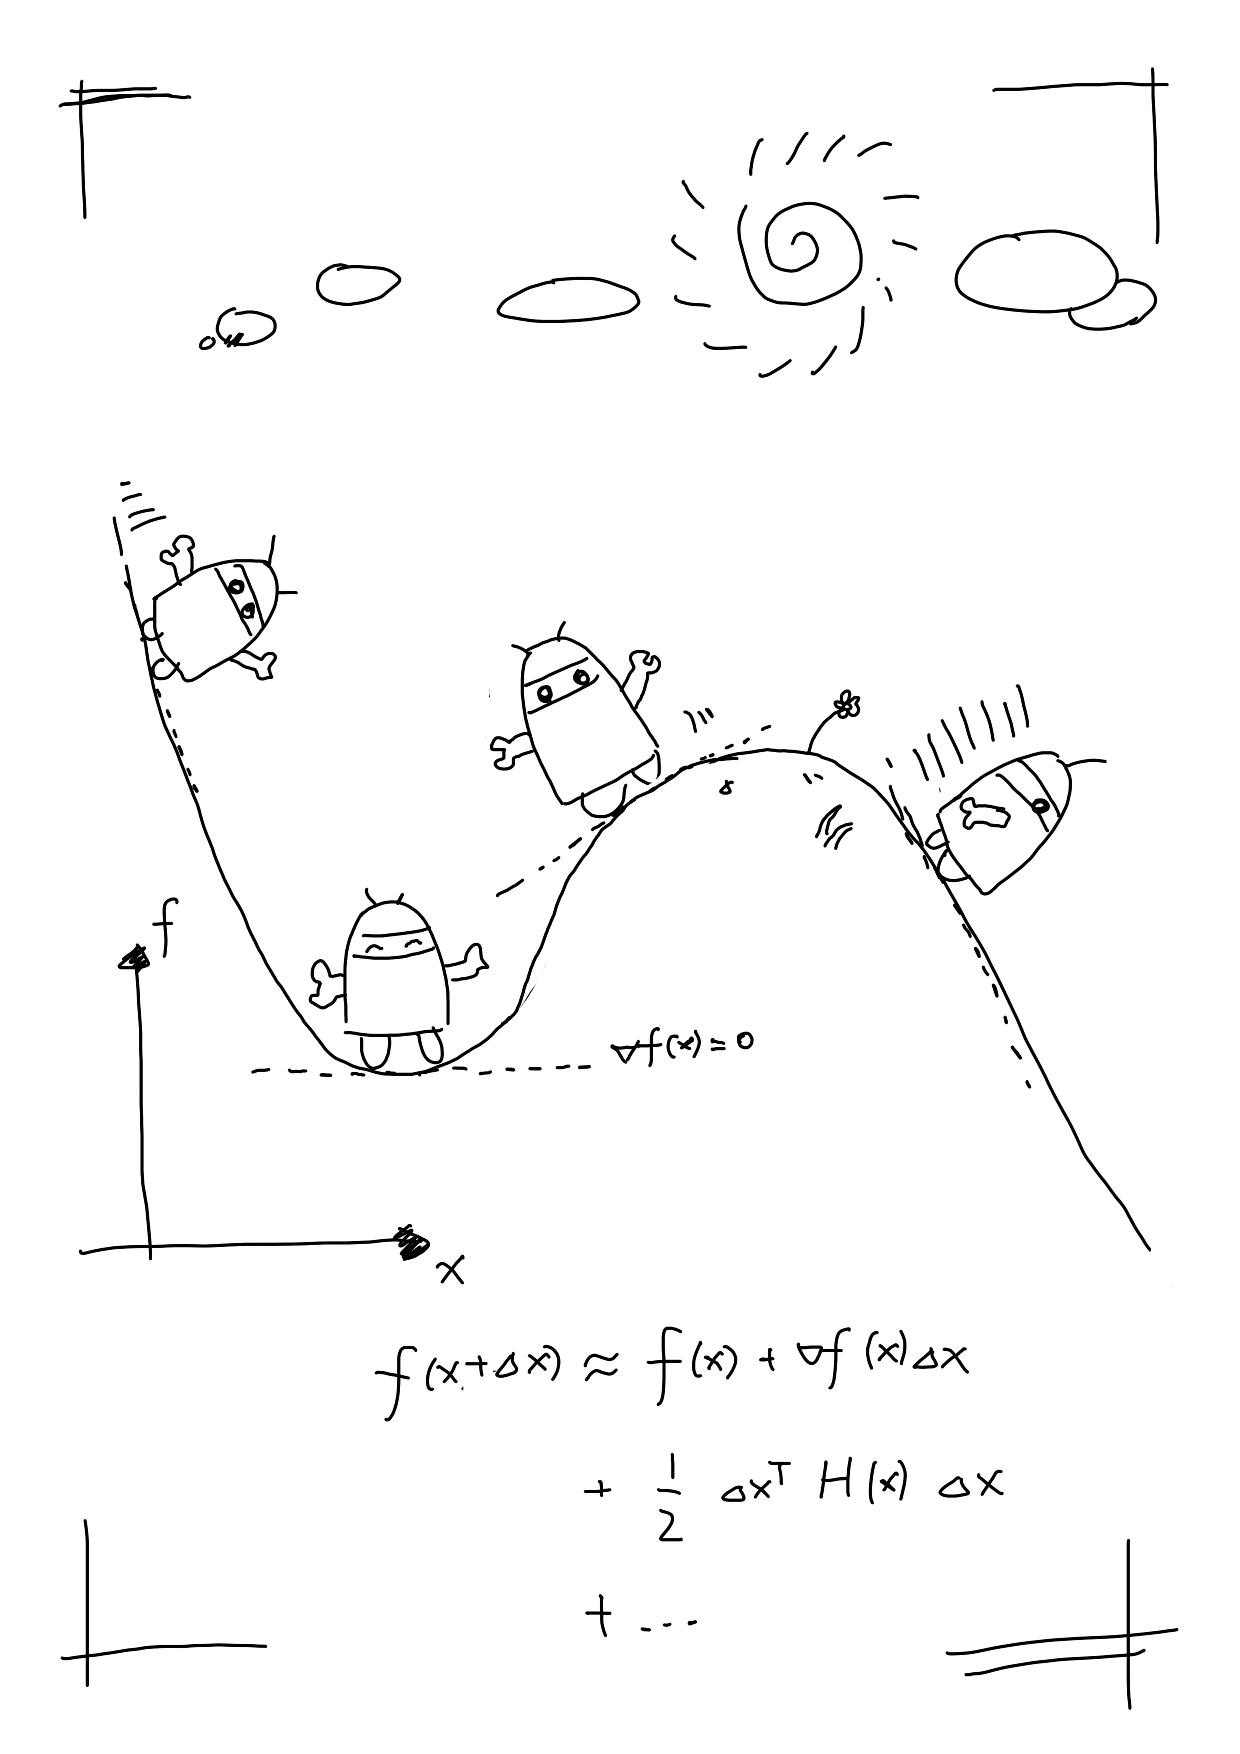
\includepdf{resources/other/ch6.pdf}

\newpage
\section{State Estimation}
\subsection{From Batch State Estimation to least-square}
According to the previous sections, the SLAM process can be described by a discrete-time motion and observation equations like~\eqref{eq:slamproblem}:
\begin{equation}
\left\{ \begin{array}{l}
{\mathbf{x}_k} = \mathbf{f}\left( {{\mathbf{x}_{k - 1}},{\mathbf{u}_k}} \right) + \mathbf{w}_k\\
{\mathbf{z}_{k,j}} = \mathbf{h}\left( {{ \mathbf{y}_j},{ \mathbf{x}_k}}  \right)+ \mathbf{v}_{k,j}
\end{array} \right. .
\end{equation}

Through the knowledge in lecture \ref{cpt:4}, we learned that $ \mathbf {x} _k $ is the pose of the camera, which can be described by $ \mathrm {SE} (3) $. As for the observation equation, we have already explained in lecture \ref{cpt:5} that it is just the pinhole camera model. To give readers a deeper impression of them, we may wish to discuss their specific parameterized form. First, the pose variable $\mathbf {x} _k $ can be expressed by $\mathbf {T} _k \in \mathrm {SE} (3) $. Second, the motion is related to the specific form of the input, but there is no particularity in visual SLAM (should be the same as ordinary robots and vehicles). We will not talk about it for now. The observation equation is given by the pinhole model. Assuming an observation of the road sign $ \mathbf {y} _j $ at $ \mathbf {x} _k $, corresponding to the pixel position on the image $ \mathbf {z} _ {k, j} $, then, observe The equation can be expressed as:
\begin{equation}
s \mathbf{z}_{k,j}= \mathbf{K} (\mathbf{R}_k {\mathbf{y}_j}+\mathbf{t}_k),
\end{equation}
where $ \mathbf {K} $ is the intrinsic matrix of the camera, and $s$ is the distance of pixels, which is also the third element of $ (\mathbf {R} _k {\mathbf {y} _j} + \mathbf {t} _k) $. If we use  transformation matrix $ \mathbf {T} _k $ to describe the pose, then the points $ \mathbf {y} _j $ must be described in homogeneous coordinates, and then converted to non-homogeneous coordinates afterwards. If you are not familiar with this process, please go back to the previous lectures.

Now, consider what happens when the data is affected by noise. In the motion and observation equations, we \textit {usually} assume that the two noise terms $ \mathbf {w} _k, \mathbf {v} _ {k, j} $ satisfy a Gaussian distribution with zero mean, like this:
\begin{equation}
{\mathbf{w}_k} \sim \mathcal{N}\left( {\mathbf{0},{\mathbf{R}_k}} \right),{\mathbf{v}_k} \sim \mathcal{N}\left( {\mathbf{0},{{{\mathbf{Q}}}_{k,j}}} \right),
\end{equation}
where $ \mathcal {N} $ means Gaussian distribution, $ \mathbf{0} $ means zero mean, and $ \mathbf {R} _k, \mathbf {Q} _ {k, j} $ is the covariance matrix. Under the influence of these noises, we hope to infer the pose $ \mathbf {x} $ and the map $ \mathbf {y} $ from the noisy data $ \mathbf {z} $ and $ \mathbf {u} $ (and their probability density distribution), which constitutes a state estimation problem.

Generally, there are two ways to deal with this state estimation problem. Since these data come gradually over time in the SLAM process, we should intuitively hold an estimated state at the current moment and then update it with new data. This method is called the \textit {incremental} method, or \textit{filtering}. For a long time in history, researchers have used filters, especially the extended Kalman filter (EKF) and its derivatives, to solve it. The other way is to record the data into a file and looking for the best trajectory and map in all time. This method is called the \textit {batch} estimation. In other words, we can collect all the input and observation data from time 0 to $ k $ together and ask, with such input and observation, how to estimate the entire trajectory and map from time 0 to $ k $?

These two different processing methods lead to many estimation methods. In general, the incremental method only cares about the state estimation of the \textit {current moment} $ \mathbf {x} _k $ but does not consider much about the previous state. Conversely, the batch method can be used to get an optimized trajectory in a long time, which is considered superior to the traditional filters \cite {Strasdat2012}, and has become the mainstream method of current visual SLAM. In extreme cases, we can let robots or drones collect data and then bring it back to the computing center for unified processing, which is also the mainstream practice of SfM (structure from motion). Of course, in these cases, the method is obviously not \textit {real-time}, which is not the most common application scenario of SLAM. So in SLAM, practical methods are usually some compromises. For example, we fix some historical trajectories and only optimize some trajectories close to the current moment, leading to the sliding window estimation method described later.

In theory, the batch method is easier to introduce. At the same time, understanding the batch method also makes it easier to understand the incremental method. Therefore, in this section, we focus on the batch optimization method based on nonlinear optimization. The Kalman filter and more in-depth knowledge will be discussed in the backend chapter. Since the batch method is discussed, we will consider all the moments from time 1 to $N$ and assume $M$ map points. Define the robot pose and map coordinates at all times as:
\[
\mathbf{x}=\{ \mathbf{x}_1, \ldots, \mathbf{x}_N \}, \quad \mathbf{y} = \{\mathbf{y}_1, \ldots, \mathbf{y}_M \}.
\]
Similarly, $ \mathbf {u} $ without subscript is used for input at all times, and $ \mathbf {z} $ is used for observation data at all times. Then we say that the state estimation of the robot, from a probabilistic point of view, is to find the state $ \mathbf {x}, \mathbf{y}$ under the condition that the input data $ \mathbf {u} $ and the observation data $\mathbf{z} $. Or, the conditional probability distribution of:
\begin{equation}
P( \mathbf{x},\mathbf{y} | \mathbf{z}, \mathbf{u}).
\end{equation}


In particular, when we do not know the control input and only have one image, that is, only considering the data brought by the observation equation, it is equivalent to estimate the conditional probability distribution $ P (\mathbf {x}, \mathbf {y} | \mathbf { z}) $. Such a problem is also called Structure from Motion (SfM), that is, how to reconstruct the three-dimensional spatial structure from images only {\cite {Agarwal2009}}.

To estimation the conditional pdf, we use the Bayes equation to switch the variables:
\begin{equation}
P\left( { \mathbf{x},\mathbf{y}| \mathbf{z}, \mathbf{u}} \right) = \frac{{P\left( {\mathbf{z},\mathbf{u}|\mathbf{x},\mathbf{y}} \right)P\left( \mathbf{x}, \mathbf{y} \right)}}{{P\left( \mathbf{z},\mathbf{u}\right)}} \propto \underbrace{P\left(  { \mathbf{z},\mathbf{u}| \mathbf{x},\mathbf{y} } \right)}_{\text{likehood}} \underbrace{P\left( \mathbf{x},\mathbf{y} \right)}_{\text{prior}}.
\end{equation}

The left side is called \textit {posterior probability}, and $ P (\mathbf {z} | \mathbf {x}) $ on the right is called \textit {likelihood} (or likehood), and the other part is $ P (\mathbf {x}) $ is called \textit {prior}. \textit {It is normally difficult to find the posterior distribution directly (in nonlinear systems), but it is feasible to find an optimal point which maximize the posterior} (Maximize a Posterior, MAP):
\begin{equation}
{(\mathbf{x},\mathbf{y})^*}_{\mathrm{MAP}} = \arg {\mathop{\rm max}\nolimits} P \left( {\mathbf{x},\mathbf{y}|\mathbf{z},\mathbf{u}} \right) = \arg \max P(\mathbf{z},\mathbf{u}|\mathbf{x},\mathbf{y})P(\mathbf{x},\mathbf{y}).
\end{equation}

Please note that the denominator part of Bayes' rule has nothing to do with the state $ \mathbf {x}, \mathbf {y} $ to be estimated, so it can be just ignored. Bayes' rule tells us that solving the maximum posterior probability is \textit {equivalent to the estimate the product of maximum likelihood and a priori}. Further, we can also say, ``I'm sorry, I don't know in prior where the robot pose or the map points are'', then there is no \textit {prior}. In this case, we can solve the \textit {Maximize Likelihood Estimation} (MLE):
\begin{equation}
{ (\mathbf{x},\mathbf{y})^*}_{\mathrm{MLE}} = \arg \max P( \mathbf{z},\mathbf{u}| \mathbf{x},\mathbf{y}).
\end{equation}

Intuitively speaking, likelihood refers to ``what observation data may be generated in the current pose''. Since we know the observation data, the maximum likelihood estimation can be understood as: ``under what state, it is most likely to produce the data currently observed''. 

\subsection{Introduction to least-squares}
Now we have formulated the state estimation problem into a MAP/MLE problem, and the next question is how to solve it. Under the assumption of Gaussian distribution, we can have a simpler form of the maximum likelihood problem. Looking back at the observation model, for a certain kind of observation, we have:
\[
{\mathbf{z}_{k,j}} = h\left( {{ \mathbf{y}_j},{ \mathbf{x}_k}} \right)+ \mathbf{v}_{k, j},
\]
Since we assume the noise item is Gaussian, which means ${\mathbf{v}_k} \sim \mathcal{N}\left( {\mathbf{0},{{{\mathbf{Q}}}_{k,j}}} \right)$, so the conditional probability of the observation data is:
\[
P( \mathbf{z}_{j,k} | \mathbf{x}_k, \mathbf{y}_j) = N\left( h(\mathbf{y}_j, \mathbf{x}_k), \mathbf{Q}_{k,j} \right),
\]
which is, of course, still a Gaussian distribution. Now let's consider solving the maximum likelihood estimation under this single observation.

We can rewrite this maximum problem into a \textit{minimum of negative logarithm} one. Gaussian distributions have better mathematical forms under negative logarithm. Consider an arbitrary multi-dimensional Gaussian distribution $\mathbf{x} \sim \mathcal{N}(\mathbf{\mu}, \boldsymbol{\Sigma})$, its probability density function expansion form is:
\begin{equation}
	P\left( \mathbf{x} \right) = \frac{1}{{\sqrt {{{(2\pi )}^N}\det (\boldsymbol{\Sigma} )} }}\exp \left( {-\frac{1}{2}{{\left( {\mathbf{x}-\mathbf{\mu}} \right)}^T}{ \boldsymbol{\Sigma} ^ {-1}}\left( {\mathbf{x}-\mathbf{\mu}} \right)} \right).
\end{equation}
Take the negative logarithm of both sides:
\begin{equation}
	-\ln \left( {P\left( \mathbf{x} \right)} \right) = \underbrace{\frac{1}{2}\ln \left( {{{\left( {2\pi} \right )}^N}\det \left( \boldsymbol{\Sigma} \right)} \right)}_{\text{discarded}} + \frac{1}{2}{\left( {\mathbf{x}-\mathbf{\mu}} \right)^T}{\boldsymbol{\Sigma} ^{-1}}\left( {\mathbf{x}-\mathbf{\mu}} \right).
\end{equation}

Because the logarithm function is monotonically increasing, maximizing the original function is equivalent to minimizing the negative logarithm. When minimizing $\mathbf{x}$ in the above formula, the first term has nothing to do with $\mathbf{x}$ and can be omitted. Therefore, as long as the quadratic term on the right is minimized, the state's maximum likelihood estimate is obtained. Substituting into the SLAM observation model, it is equivalent to find such a solution:

\begin{equation}
	\begin{aligned}
		(\mathbf{x}_k,\mathbf{y}_j)^* &= \arg \max \mathcal{N}(h(\mathbf{y}_j, \mathbf{x}_k), \mathbf{Q }_{k,j}) \\ &= \arg \min \left( {{{\left( {{ \mathbf{z}_{k,j}}-h\left( {{\mathbf{x }_k},{\mathbf{y}_j}} \right)} \right)}^T} \mathbf{Q}_{k,j}^{-1}\left( {{\mathbf{z}_{k,j}}-h\left( {{\mathbf{x}_k},{\mathbf{y}_j}} \right)} \right)} \right).
	\end{aligned}
\end{equation}

We found that this equation is equivalent to a quadratic form that minimizes the noise term (i.e., the error). This quadratic form is called \textit{Mahalanobis distance}. It can also be regarded as the Euclidean distance ($\mathcal{L}_2$-norm) weighted by $\mathbf{Q}_{k,j}^{-1}$, where $\mathbf{Q}_{k,j} ^{-1}$ is also called the \textit{information matrix}, which is exactly the \textit{inverse} of the Gaussian covariance matrix.

Now we put all the observations together. It is usually assumed that the inputs and observations are independent of each other, which means that each input is independent, each observation is independent, and input and observation are still independent. So we can factorize the joint distribution like this:
\begin{equation}
	P\left( {\mathbf{z},\mathbf{u}|\mathbf{x},\mathbf{y}} \right) = \prod\limits_k {P\left( {{\mathbf{u}_k }|{\mathbf{x}_{k-1}},{\mathbf{x}_k}} \right)} \prod\limits_{k,j} {P\left( {{\mathbf{z} _{k,j}}|{\mathbf{x}_k},{\mathbf{y}_j}} \right)},
\end{equation}

It shows that we can handle the movement and observation at each moment independently. Let's define the error between the model and real data: 
\begin{equation}
	\begin{array}{l}
		{\mathbf{e}_{u,k}} = {\mathbf{x}_k}-f\left( {{\mathbf{x}_{k-1}},{\mathbf{u}_k} } \right)\\
		{\mathbf{e}_{z,j,k}} = {\mathbf{z}_{k,j}}-h\left( {{\mathbf{x}_k},{\mathbf{y} _j}} \right),
	\end{array}
\end{equation}
Then, minimizing the Mahalanobis distance between the estimated value and the measurements from sensors is equivalent to finding the maximum likelihood estimation. The negative logarithm allows us to turn the product into a summation:
\begin{equation}
	\label{eq:least-square}
	\min J (\mathbf{x},\mathbf{y}) = \sum\limits_k {\mathbf{e}_{u,k}^T \mathbf{R}_k^{-1} {\mathbf{e}_{u,k}}} + \sum\limits_k {\sum\limits_j {\mathbf{e}_{z,k,j}^T \mathbf{Q}_ {k,j}^{-1}{\mathbf{e}_{z,k,j}}}}.
\end{equation}
In this way, a \textit{least-square problem} is obtained with the same solution as the MLE problem. Intuitively speaking, due to the presence of noise, when we substitute the estimated trajectory and map into the SLAM motion and observation models, they will not be perfectly fit. What shall we do at this time? We perform \textit{fine-tuning} on the state's estimated value so that the overall error is reduced. Of course, finally, we will reach a (local) \textit{minimum value}. This is a typical nonlinear optimization process.

Observing the formula~\eqref{eq:least-square} carefully, we find that the least-squares problem in SLAM has some specific structures:

\begin{itemize}
	\item First, the objective function of the whole problem consists of many (weighted) error quadratic forms. Although the overall state variable's dimensionality is very high, each error term is simple and is only related to one or two state variables. For example, the motion error is only related to $\mathbf{x}_{k-1}, \mathbf{x}_k$, and the observation error is only related to $\mathbf{x}_k, \mathbf{y}_j$. This relationship will give a \textit{sparse} least-square problem, which we will investigate further in the backend chapter.
	\item Secondly, if you use Lie algebra to represent the increment, the problem is the least-squares problem of \textit{unconstrained}. However, if the rotation matrix/transformation matrix is ​​used to describe the pose, the constraint of the rotation matrix itself will be introduced, that is, ``$\mathrm{s.t.}\ \mathbf{R}^T \mathbf{R} = \mathbf{I}$ and $\det (\mathbf{R})=1$ '' need to be added to the problem. Additional constraints can make optimization more difficult.
	\item Finally, we used a quadratic metric error, exactly the $\mathcal{L}_2-$norm. The information matrix is used as the weights of each element. For example, if an observation is very accurate, the covariance matrix will be ``small'' and the information matrix will be ``large'', so this error term will have a higher weight than the others in the whole problem. We will see some drawbacks of the $\mathcal{L}_2$ error later.
\end{itemize}

Next, we will introduce how to solve this least-squares problem, which requires some basic knowledge of nonlinear optimization. In particular, we want to discuss how to solve such a general unconstrained nonlinear least-squares problem. In the following lectures, we will make extensive use of this lecture's results and discuss its application in the SLAM's front and backends.

\subsection{Example: Batch State Estimation}
Maybe it's better to give an example here. Consider a very simple discrete-time system:
\begin{equation}
    \begin{array}{lll}
        {x_k} &= {x_{k-1}} + {u_k} + {w_k},&\qquad w_k \sim \mathcal{N}\left( {0,Q_k} \right)\\
        {z_k} &= {x_k} + {n_k},&\qquad {n_k}\sim \mathcal{N}\left( {0,R_k} \right)
    \end{array},
\end{equation}
which describes a car moving forward or backward along the $x$ axis. The first formula is the motion model, where $u_k$ is the input, and $w_k$ is the noise; the second formula is the observation model, where $z_k$ is the measurement of the position. We set the time $k=1,\ldots,3$, and want to estimate the states based on the existing $v,y$. Suppose the initial state $x_0$ is known. Let's derive the maximum likelihood estimation of the batch state estimation.

First, let the batch state variable be $\mathbf{x} = [x_0,x_1, x_2, x_3]^T$, and the batch observation be $\mathbf{z} = [z_1,z_2,z_3]^T$, define $\mathbf{u}=[u_1,u_2,u_3]^T$ in the same way. According to the previous derivation, we know that the maximum likelihood estimate is:
\begin{equation}
    \begin{aligned}
        {\mathbf{x}_{\mathrm{map}}^*} &= \arg \max P(\mathbf{x}|\mathbf{u},\mathbf{z}) = \arg \max P( \mathbf{u},\mathbf{z}|\mathbf{x})\\
        &= \prod\limits_{k = 1}^3 {P({u_k}|{x_{k-1}},{x_k})\prod\limits_{k = 1}^3 {P\left( { {z_k}|{x_k}} \right)} },
    \end{aligned}
\end{equation}
For each item, such as the motion equation, we have:
\begin{equation}
    P({u_k}|{x_{k-1}},{x_k}) = \mathcal{N}({x_k}-{x_{k-1}},{Q_k}).
\end{equation}
The observation equation is similar:
\begin{equation}
    P\left( {{z_k}|{x_k}} \right) = \mathcal{N}\left( {{x_k},{R_k}} \right).
\end{equation}
According to the previous statements, the error variable can be constructed as:
\begin{equation}
    {e_{u,k}} = {x_k}-{x_{k-1}}-{u_k}, \quad {e_{z,k}} = {z_k}-{x_k},
\end{equation}
Then the objective function of the least-squares is:
\begin{equation}
    \min \sum\limits_{k = 1}^3 {e_{u,k}^T Q_k^{-1}{e_{u,k}}} + \sum\limits_{k = 1 }^3 {e_{z,k}^T{R^{-1}_k}{e_{z,k}}}.
\end{equation}

In addition, since this system is a linear one, we can easily write the equations in the vector/matrix form. Define the vector $\mathbf{y}=[\mathbf{u}, \mathbf{z}]^T$, then the error can be defined as:
\begin{equation}
    \mathbf{y}-\mathbf{H}\mathbf{x} = \mathbf{e} \sim \mathcal{N}(\mathbf{0}, \boldsymbol{\Sigma}),
\end{equation}
where
\begin{equation}
    \mathbf{H} = \left[ {\begin{array}{*{20}{c}}
            1&{-1}&0&0\\
            0&1&{-1}&0\\
            0&0&1&{-1}\\
            \hline
            0&1&0&0\\
            0&0&1&0\\
            0&0&0&1
    \end{array}} \right],
\end{equation}
and $\boldsymbol{\Sigma}=\mathrm{diag}(Q_1, Q_2, Q_3, R_1, R_2, R_3)$. The whole question can be written as:
\begin{equation}
    \mathbf{x}^*_{\mathrm{map}} = \arg \min \mathbf{e}^T \boldsymbol{\Sigma}^{-1} \mathbf{e},
\end{equation}
Later we will see that this problem has a unique solution:
\begin{equation}
    \mathbf{x}^*_{\mathrm{map}} = (\mathbf{H}^T \boldsymbol{\Sigma}^{-1} \mathbf{H})^{-1} \mathbf{H}^T \boldsymbol{\Sigma}^{-1} \mathbf{y},
\end{equation}
since $(\mathbf{H}^T \boldsymbol{\Sigma}^{-1} \mathbf{H})^{-1}$ is invertible.

\section{Nonlinear Least-square Problem}
\label{sec:6.2}
First, consider a simple least-square problem:
\begin{equation}
    \mathop {\min }\limits_{\mathbf{x}} F(\mathbf{x}) = \frac{1}{2}{\left\| {f\left( \mathbf{x} \right) } \right\|^2_2},
\end{equation}
where the state variable is $\mathbf{x} \in \mathbb{R}^n$, and $f$ is any scalar nonlinear function $f(\mathbf{x}): \mathbb{R}^n \mapsto \mathbb{R}$. Note that the coefficient $\frac{1}{2}$ here is not important. Some literature has this coefficient, and some not. It will not affect the subsequent conclusions. Obviously, if $f$ is a mathematically simple function, then the problem can be solved in an analytical form. Let the derivative of the objective function be zero, and then find the optimal value of $\mathbf{x}$, just like finding the extreme value of a scalar function:
\begin{equation}
    \frac{ \mathrm{d} F}{ \mathrm{d} \mathbf{x}} = \mathbf{0}.
\end{equation}

We reach the minimum, maximum, or saddle points by solving this equation (or, intuitively, by letting the derivative be zero). But is this equation easy to solve? Well, it depends on the form of the derivative function of $f$. If $f$ is just a simple linear function, then the problem is only a simple linear least-square problem. But, some derivative functions may be complicated in form, making the equation difficult to solve. Solving this equation requires us to know the \textit{global property} of the objective function, which is usually not possible. For the least-square problem that is inconvenient to solve directly, we can use the \textit{iterated methods} to start from an initial value and continuously update the current estimations to reduce the objective function. The specific steps can be listed as follows:
\begin{mdframed}  
    \begin{enumerate}
        \item Give an initial value $\mathbf{x}_0$.
        \item For $k$-th iteration, we find an incremental value of $\Delta \mathbf{x}_k$, such that the object function $\left\| {f\left( \mathbf{x}_k + \Delta \mathbf{x}_k \right)} \right \|^2_2$ reaches a smaller value.
        \item If $\Delta \mathbf{x}_k$ is small enough, stop the algorithm.
        \item Otherwise, let $\mathbf{x}_{k+1} = \mathbf{x}_k+\Delta \mathbf{x}_k$ and return to step 2.
    \end{enumerate}
\end{mdframed}

Now things get much simpler. We turn the problem of solving the derivative function equals zero into a problem of looking for decreasing increments $\Delta \mathbf{x}_k$. We will see that since the objective function can be linearly approximated at the current estimation, the increment calculation will be more straightforward \footnote{Linear cases are always the easiest ones.}. When the function decreases until the increment becomes very small, it is considered that the algorithm converges, and the objective function reaches a minimum value. In this process, the problem is how to find the increment at each iteration point, which is a local problem. We only need to be concerned about the local properties of $f$ at the iteration value rather than the global properties. Such methods are widely used in optimization, machine learning, and other fields.

Next, we examine how to find this increment $\Delta \mathbf{x}_k$. This part of knowledge belongs to the field of numerical optimization. Let's take a quick look at some widely used results.

\subsection{The First and Second-order Method}
Now consider the $k$-th iteration. Suppose we are at $\mathbf{x}_k$ and want to find the increment $\Delta \mathbf{x}_k$, then the most intuitive way is to make the Taylor expansion of the objective function in $\mathbf{x}_k$:
\begin{equation}
    F(\mathbf{x}_k+\Delta \mathbf{x}_k) \approx F{\left( \mathbf{x}_k \right)} + \mathbf{J} \left( \mathbf{x}_k \right) ^T \Delta \mathbf{x}_k + \frac{1}{2}\Delta {\mathbf{x}_k^T}\mathbf{H}(\mathbf{ x}_k) \Delta \mathbf{x}_k,
\end{equation}
where $\mathbf{J}(\mathbf{x}_k)$ is the first derivative of $F(\mathbf{x})$ with respect to $\mathbf{x}$ (also called gradient, \textit{Jacobi} Matrix, or \textit{Jacobian}) \footnote{We write $\mathbf{J}(\mathbf{x})$ as a column vector, then it can be inner product with $\Delta \mathbf{x}$ to get a scalar. }, $\mathbf{H}$ is the second-order derivative (or \textit{Hessian}), which are all taken at $\mathbf{x}_k$. Readers should be familiar with them in the undergraduate course like multivariate calculus. We can choose to keep the first-order or second-order terms of the Taylor expansion, and the corresponding solution is called the first-order or the second-order method. In the simplest way, if we only keep the first-order one, then taking the increment at the minus gradient direction will ensure that the function decreases: 
\begin{equation}
    \Delta \mathbf{x}^* =-\mathbf{J}(\mathbf{x}_k).
\end{equation}

Of course, this is only a direction. Usually, we have to compute another step length parameter, say, $\lambda$. The step length can be calculated according to certain conditions {\cite{Wolfe1969}}. There are also some empirical methods in machine learning, but we will not discuss them. This method is called \textit{steepest descent method}. Its intuitive meaning is very simple. As long as we move along the reverse gradient direction, the objective function must decrease if the first-order (linear) approximation still holds.

Note that the above discussion was carried out during the $k$-th iteration and did not involve any information about $k$. To simplify the notation, we will omit the subscript $k$ later and think that these discussions are valid for each iteration.

On the other hand, we can choose to keep the second step information, and the increment equation is:
\begin{equation}
    \Delta \mathbf{x}^* = \arg \min \left(F\left( \mathbf{x} \right) + \mathbf{J} \left( \mathbf{x} \right)^T \Delta \mathbf{x} + \frac{1}{2}\Delta {\mathbf{x}^T}\mathbf{H} \Delta \mathbf{x} \right).
\end{equation}
The right side only contains the zero-order, first-order and quadratic terms of $\Delta \mathbf{x}$. Finding the derivative of $\Delta \mathbf{x}$ on the right side of the equation and setting it to zero leads to: \footnote{For students who are not familiar with matrix derivation, please refer to appendix \ref{cpt:app-B}. }
\begin{equation}
    \label{eq:newton-method}
    \mathbf{J} + \mathbf{H} \Delta \mathbf{x} = \mathbf{0} \Rightarrow
    \mathbf{H} \Delta \mathbf{x} = -\mathbf{J}.
\end{equation}

We can also solve this linear equation and get the increment. This method is also called \textit{Newton's method}.

We have seen that both the first-order and second-order methods are very intuitive, as long as we can calculate the Taylor expansion of $f$ and find the increments. We say, hey, the function looks like a linear or quadratic one. We can use the approximated function's minimum value to guess the minimum value of the original function. As long as the original objective function really looks like a first-order or quadratic function locally, this type of algorithm is always valid (this is also the most cases in reality). However, these two methods also have their drawbacks. The steepest descent method is too greedy and easy to lead a zigzag way and increases the number of iterations. However, Newton's method needs to calculate the $\mathbf{H}$ matrix of the objective function, which is very time-expensive when the problem is large. We usually tend to avoid the calculation of $\mathbf{H}$. For general problems, some quasi-Newton methods can get better results. For least-square problems, there are several more practical methods: the \textit{Gauss-Newton's method} and the (Levernburg-Marquardt's method).

\subsection{The Gauss-Newton Method}
The Gauss-Newton method is one of the simplest methods in optimization algorithms. Its idea is to carry out a first-order Taylor expansion of $f(\mathbf{x})$. Please note that this is not the objective function $F(\mathbf{x})$ but the lower case $f(\mathbf{x})$, otherwise it is the same as Newton's method.
\begin{equation}
    \label{eq:approximation}
    f\left( {\mathbf{x} + \Delta \mathbf{x}} \right) \approx f\left( \mathbf{x} \right) + \mathbf{J} \left( \mathbf{x} \right)^T \Delta \mathbf{x}.
\end{equation}

Here $\mathbf{J}(\mathbf{x})$ is the derivative of $f(\mathbf{x})$ with respect to $\mathbf{x}$, which is a column vector of $n \times 1$. According to the previous framework, the current goal is to find the increment $\Delta \mathbf{x}$ such that $\left\| {f\left( \mathbf{x} + \Delta \mathbf{x} \right)} \right \|^2$ reached the minimum. In order to find $\Delta \mathbf{x}$, we need to solve a linear least-square problem \footnote{We omit the information matrix to simplify the derivation here.}:
\begin{equation}
    \Delta \mathbf{x}^* = \arg \mathop {\min }\limits_{\Delta \mathbf{x}} \frac{1}{2}{\left\| {f\left( \mathbf{x} \right) + \mathbf{J} \left( \mathbf{x} \right)^T \Delta \mathbf{x} } \right\|^2}.
\end{equation}
    
What's the difference from before? According to the extreme conditions, we set the derivative with $\Delta \mathbf{x}$ to zero to reach the extreme value. To do this, let's first expand the square term of the objective function:
\begin{align*}
    \frac{1}{2}{\left\| {f\left( \mathbf{x} \right) + \mathbf{J} \left( \mathbf{x} \right)^T \Delta \mathbf{x}} \right\|^2} &= \frac{1}{2}{\left( {f\left( \mathbf{x} \right) + \mathbf{J}\left( \mathbf{x} \right)^T \Delta \mathbf{x}} \right)^T}\left( {f\left( \mathbf{x} \right) + \mathbf{J} \left( \mathbf{x} \right)^T \Delta \mathbf{x}} \right)\\
    &= \frac{1}{2}\left( \| f{{\left( \mathbf{x} \right)}\|^2_2 + 2 f\left( \mathbf{x} \right) \mathbf{J} {{\left( \mathbf{x} \right)}}^T \Delta \mathbf{x} + \Delta { \mathbf{x}^T}{\mathbf{J} (\mathbf{x})} \mathbf{J}(\mathbf{x})^T \Delta \mathbf{x}} \right).
\end{align*}


Find the derivative of the above formula with respect to $\Delta \mathbf{x}$ and set it to zero:
\begin{displaymath}
    \mathbf{J} {\left( \mathbf{x} \right)}f\left( \mathbf{x} \right) + \mathbf{J} {\left( \mathbf{x} \right)} \mathbf{J}^T \left( \mathbf{x} \right)\Delta \mathbf{x} = \mathbf{0}.
\end{displaymath}

The following equation can be obtained:
\begin{equation}
    \underbrace{\mathbf{J} {\left( \mathbf{x} \right)} \mathbf{J}^T}_{\mathbf{H}(\mathbf{x})} \left( \mathbf{x} \right)\Delta \mathbf{x} =  \underbrace{- \mathbf{J} {\left( \mathbf{x} \right)} f\left( \mathbf{x} \right)}_{\mathbf{g}(\mathbf{x})}.
\end{equation}

This equation is a \textit{linear equation} of the variable $\Delta \mathbf{x}$. We call it \textit{normal equation} or \textit{Gauss-Newton equation}. We define the coefficients on the left as $\mathbf{H}$ and the coefficient on the right as $\mathbf{g}$, then the above formula becomes:
\begin{equation}
    \label{eq:minimize-deltax}
    \mathbf{H} \Delta \mathbf{x} = \mathbf{g}.
\end{equation}
It makes sense to mark the left side as $\mathbf{H}$ here. Compared with Newton's method~\ref{eq:newton-method}, Gauss-Newton's method uses $\mathbf{J}\mathbf{J}^T$ \textit{as the approximation} of the second-order Hessian matrix in Newton's method, thus omitting the calculation of $\mathbf{H}$. Please note that solving the normal equation is the core of the entire optimization problem. If we can get the $\Delta \mathbf{x}$ in each iteration, then the algorithm of the Gauss-Newton method can be written as:

\begin{mdframed}
    \begin{enumerate}
        \item Set it initial value as $\mathbf{x}_0$.
        \item For $k$-th iteration, calculate the Jacobian $\mathbf{J}(\mathbf{x}_k)$ and residual $f(\mathbf{x}_k)$.
        \item Solve the normal equation: $\mathbf{H} \Delta \mathbf{x}_k = \mathbf{g}$.
        \item If $\Delta \mathbf{x}_k$ is small enough, stop the algorithm. Otherwise let $\mathbf{x}_{k+1} = \mathbf{x}_k+\Delta \mathbf{x}_k$ and return to step 2.
    \end{enumerate}
\end{mdframed}

It can be seen from the algorithm steps that the solution of the incremental equation occupies the major position. As long as we can solve the increment smoothly, we can ensure that the objective function decreases correctly.

In order to solve the incremental equation, we need to solve $\mathbf{H}^{-1}$, which requires the $\mathbf{H}$ matrix to be invertible. However, the calculated $\mathbf{J} \mathbf{ J}^T$ is only semi-positive definite. If $\mathbf{J}$ has null-spaces, which means we can find non-zero $\Delta \mathbf{x}$ such that $\mathbf{J} \Delta\mathbf{x} = \mathbf{0}$, then we can not determine which $\Delta \mathbf{x}$ can really makes the objective function decreases. In that case, the algorithm is probably not converging, and we may obtain erroneous results. Intuitively, the local approximation of the original function at this point is not like a quadratic function. Furthermore, even if we assume that $\mathbf{H}$ is not singular or ill-conditioned, but if we take a very large step size $\Delta \mathbf{x}$, the result can still be bad since linear approximation is not accurate enough at that point. So in practice, we can't guarantee that the Gauss-Newton method converges. Sometimes they can reach even larger objective function values than the initial one. 

Although the Gauss-Newton method has these shortcomings, it is still a simple and effective method for nonlinear optimization, and it is worth learning. In nonlinear optimization, quite a lot of algorithms can be taken as the Gauss-Newton method's variants. These algorithms all use the idea of the Gauss-Newton method and correct their shortcomings through their own improvements. For example, some \textit{line search method} adds an extra step size $\alpha$. After determining $\Delta \mathbf{x}$, we may further find the $\alpha$ to make $\left\| f (\mathbf{x} + \alpha \Delta \mathbf{ x}) \right\|^2$ is minimized, instead of simply making $\alpha = 1$.

The Levenberg-Marquardt method corrects these problems to a certain extent. It is generally considered more robust than the Gauss-Newton method, but its convergence rate may be slower than the Gauss-Newton method. Such a kind of method is also called as \textit{damped Newton Method}.

\subsection{The Levernberg-Marquatdt Method}
The approximate second-order Taylor expansion used in the Gauss-Newton method can only have a good approximation effect near the expansion point. So, we naturally thought a range should be added to $\Delta \mathbf{x}$, called \textit{trust-region}. This range defines under what circumstances the second-order approximation is valid. This type of method is also called \textit{trust-region method}. We think the approximation is valid only in the trusted region; otherwise, it may go wrong if the approximation goes outside.

So how to determine the scope of this trust-region? A good method is to determine it based on the difference between our approximate model and the real object function: if the difference is small, it means that the approximation is good, and we may expand the trust-region; conversely, if the difference is large, we will reduce the range of approximation. We define an indicator $\rho$ to describe the degree of approximation:
\begin{equation}\label{eq:6.24}
	\rho = \frac{{f\left( {\mathbf{x} + \Delta \mathbf{x}} \right)}-{{ {f\left( \mathbf{x} \right)} }}} {\mathbf{J}\left( \mathbf{x} \right)^T \Delta \mathbf{x}}.
\end{equation}
The numerator of $\rho$ is the decreasing value of the real object function, and the denominator is the decreasing value of the approximate model. If $\rho$ is close to 1, we may say the approximation is good. A small $\rho$ is indicating that the actual reduced value is far less than the approximate reduced value. The approximation is poor in this case, and the trust-region needs to be reduced. Conversely, if $\rho$ is relatively large, it means that the actual decline is greater than expected, and we can enlarge the approximate range.

Therefore, we build an improved version of the nonlinear optimization framework, which will have a better effect than the Gauss-Newton method:

\begin{mdframed}
	\begin{enumerate}
		\item Give the initial value $\mathbf{x}_0$ and initial trust-region radius $\mu$.
		\item For $k$-th iteration, we solve a linear problem based on Gauss-Newton's method added with a trust-region: 
		\begin{equation}\label{eq:LM}
			\mathop {\min }\limits_{\Delta \mathbf{x}_k} \frac{1}{2}{\left\| {f\left( \mathbf{x}_k \right) + \mathbf{J} \left( \mathbf{x}_k \right)^T \Delta \mathbf{x}_k} \right\|^2}, \quad \mathrm{s.t.}\quad {\left\| {\mathbf{D} \Delta \mathbf{x}_k} \right\|^2} \leqslant \mu ,
		\end{equation}
		where $\mu$ is the radius and $\mathbf{D}$ is a coefficient matrix, which will be discussed in below. 
		\item Compute $\rho$ using equation \eqref{eq:6.24}. 
		\item If $\rho > \frac{3}{4}$, set $\mu = 2 \mu$. 
		\item Otherwise, if $\rho < \frac{1}{4}$, set $\mu = 0.5 \mu$. 
		\item If $\rho$ is larger than a given threshold, set $\mathbf{x}_{k+1} = \mathbf{x}_k+\Delta \mathbf{x}_k$. 
		\item Go back to step 2 if not converged, otherwise return the result. 
	\end{enumerate}
\end{mdframed}

Here, the range expansion's multiply factor and thresholds are empirical values and can be replaced with other values. In the formula \eqref{eq:LM}, we limit the increment to a sphere with a radius of $\mu$ and think that it is valid only in this sphere. After bringing into the $\mathbf{D}$, this sphere can be seen as an ellipsoid. In the optimization method proposed by Levenberg, taking $\mathbf{D}$ into the unit matrix $\mathbf{I}$ is equivalent to directly constraining $\Delta \mathbf{x}_k$ in a sphere. Subsequently, Marquardt proposed to take $\mathbf{D}$ as a non-negative diagonal matrix. In practice, the square root of the diagonal elements of $\mathbf{J}^T \mathbf{J}$ is usually used as $\mathbf{D}$ so that the constraint range is larger on the dimensions with small gradient.

In any case, in Levenberg-Marquardt optimization, we need to solve a sub-problem like \eqref{eq:LM} to obtain the gradient. This sub-problem is an optimization problem with inequality constraints. We use Lagrangian multipliers to put the constraints in the objective function to form the Lagrangian function:
\begin{equation}
    \mathcal{L}(\Delta \mathbf{x}_k, \lambda)= \frac{1}{2} {\left\| {f\left( \mathbf{x}_k \right) + \mathbf{J} \left( \mathbf{x}_k \right)^T \Delta \mathbf{x}_k} \right\|^2} + \frac{\lambda}{2} \left( \left\| \mathbf{D} \Delta \mathbf{x}_k \right\|^2 - \mu \right),
\end{equation}
where $\lambda$ is the Lagrange multiplier. Similar to the method in the Gauss-Newton, let the derivative of the Lagrangian function with respect to $\Delta \mathbf{x}$ be zero, and we still need to solve the linear equation for calculating the increment:
\begin{equation}
    \left( \mathbf{H} +\lambda \mathbf{D}^T \mathbf{D} \right) \Delta \mathbf{x}_k = \mathbf{g}.
\end{equation}

It can be seen that the incremental equation has an extra $\lambda \mathbf{D}^T \mathbf{D}$ compared to the Gauss-Newton method. If you consider its simplified form $\mathbf{D}=\mathbf{I}$, then it is equivalent to solving \footnote{Strict readers may not be satisfied with the description here. In addition to the Lagrangian function derivation to zero, the KKT condition also has some other constraints: $\lambda>0$, and $\lambda(\|\mathbf{D} \Delta \mathbf{x}\|^2-\mu)=0$. But in the L-M iteration, we might as well regard it as a penalty term (augmented Lagrangian) with $\lambda$ as the weight on the objective function of the original problem. After each iteration, if the trust-region condition is not satisfied, or the objective function increases, the weight of $\lambda$ is increased until the trust-region condition is finally satisfied. Therefore, there are different interpretations of the L-M algorithm in theory, but we only care about whether it works smoothly in practice. }:
\begin{displaymath}
    \left( \mathbf{H} +\lambda \mathbf{I} \right) \Delta \mathbf{x}_k = \mathbf{g}.
\end{displaymath}

We can see that when the parameter $\lambda$ is relatively small, $\mathbf{H}$ dominates the normal equation, which shows that the quadratic approximation model is better in this range. The Levenberg-Marquardt method is more close to the Gauss-Newton method. On the other hand, when $\lambda$ is relatively large, $\lambda \mathbf{I}$ occupies a dominant position. The Levenberg-Marquardt method is closer to the one-step descent method (the steepest descent), which means that the quadratic approximation is not good enough. The solution method of the Levenberg-Marquardt method can avoid the non-singular and ill-conditioned problems of the coefficient matrix of linear equations to a certain extent and provide more stable and accurate increments $\Delta \mathbf{x} $.

In practice, there are also many other ways to solve the increment, such as Dog-Leg \cite{Nocedal2006} and other methods. What we have introduced here is just the most common and basic method, and it is also the most widely-used method in visual SLAM. We usually choose one of the Gauss-Newton or Levenberg-Marquardt methods as the gradient descent strategy in practical problems. When the problem is well-formed, Gauss-Newton is used. Otherwise, in ill-formed problems, we use the Levenberg-Marquardt method.

\subsection{Conclusion}
Since I don't want this book to become a headache-inducing mathematics textbook, only two of the most common nonlinear optimization schemes are listed here: the Gauss-Newton method and the Levenberg-Marquardt method. We avoided many discussions of mathematical properties. If readers are interested in optimization, you can read other books dedicated to numerical optimization (this is a big topic) like \cite{Nocedal2006}. The optimization methods represented by the Gauss-Newton method and the Levenberg-Marquardt method have been implemented and provided to users in many open-source optimization libraries. We will conduct experiments below. Optimization is an essential mathematical tool for dealing with many practical problems. It plays a central role in visual SLAM and one of the core methods for solving problems in other fields such as deep learning (the amount of deep learning data is substantial, where the first-order method is a major choice). We hope that readers can learn more about optimization algorithms based on their own capabilities.

Perhaps you have discovered that whether it is the Gauss-Newton method or the Levenberg-Marquardt method, the variable's initial value needs to be provided when doing the optimization calculation. You may ask, can this initial value be set arbitrarily? Of course not. In fact, iterative solutions of nonlinear optimization require users to provide a good initial value. Because the objective function is too complicated, it is difficult to predict the solution space change. Providing different initial values ​​for the problem often leads to different calculation results. This situation is a common problem of nonlinear optimization: most algorithms easily fall into local minima. Therefore, no matter what kind of scientific problem, we should provide the initial value carefully. For example, in the visual SLAM problem, we will use ICP, PnP, and other algorithms to provide the optimized initial value. In short, a good initial value is significant for optimization problems!

Readers may also have questions about the optimization mentioned above: how to solve the incremental linear equations? We have only mentioned that the incremental equation is linear, but does it require many calculations to invert the coefficient matrix directly? Of course not. In the visual SLAM algorithm, the dimension of $\Delta \mathbf{x}$ is often as large as hundreds or thousands. If you are doing large-scale visual 3D reconstruction, you will often find that this dimension can be easily achieved at hundreds of thousands or even higher levels. Most processors cannot afford such a large matrix inversion computation, so there are many numerical solutions for linear equations. There are different solutions in different fields, but there is almost no way to directly find the general inverse coefficient matrix. We will use matrix decomposition to solve linear equations, such as QR, Cholesky, and other decomposition methods. These methods can usually be found in textbooks, such as the matrix theory, and we will not introduce them.

Fortunately, the visual SLAM matrix has a specific sparse form, which can be solved in real-time applications. We will introduce its principle in detail in lecture \ref{cpt:backend1}. Using the sparse form of elimination, decomposition, and finally solving increment will significantly improve the solution's efficiency. In many open source optimization libraries, variables with a dimension of more than 10,000 can be solved in a few seconds or less on a general PC. The reason is that more advanced mathematical tools are used. The visual SLAM algorithm can now be implemented in real-time, thanks to the coefficient matrix is ​​sparse. If the matrix is ​​dense, I am afraid that optimization of this kind of visual SLAM algorithm will not be widely adopted by the academic community \cite{Lourakis2009, Sibley2009a, Triggs2000}.

\section{Practice: Curve Fitting}
\subsection{Curve Fitting with Gauss-Newton}
Next, we use a simple example to demonstrate how to solve the least-square problem. We will demonstrate how to write the Gauss-Newton method by hand and then introduce how to use the optimization library to solve this problem. For the same problem, these implementations will get the same result because their core algorithms are the same.

Consider a curve that satisfies the following equation:
\[
y = \exp( ax^2 + bx + c ) + w,
\]
where $a, b, c$ are the parameters of the curve, and $w$ is the Gaussian noise, satisfying $w \sim (0, \sigma^2)$. We deliberately chose such a nonlinear model so that the problem is not too easy. Now, suppose we have $N$ observation data points about $x and y$ and want to find the parameters of the curve based on these data points. Then, we solve the following least-square problem to estimate the curve parameters:
\begin{equation}
    \min \limits_{a,b,c} \frac{1}{2}\sum\limits_{i = 1}^N {{{\left\| {{y_i} - \exp \left( {ax_i^2 + bx_i + c} \right)} \right\|}^2}} .
\end{equation}

Please note that the estimated variables are $a, b, c$, not $x$. In our program, the true value of $x,y$ is generated according to the model, and then the Gaussian noise is added to the true value. Subsequently, the Gauss-Newton method was used to fit a parametric model from the noisy data. Define the error as:
\begin{equation}
    e_i = y_i - \exp \left( {ax_i^2 + bx_i + c} \right),
\end{equation}
Then we can find the derivative of each error term with respect to the state variable:
\begin{equation}
    \begin{aligned}
        \frac{{\partial {e_i}}}{{\partial a}} &=  - x_i^2\exp \left( {ax_i^2 + b{x_i} + c} \right)\\
        \frac{{\partial e_i}}{{\partial b}} &=  - {x_i}\exp \left( {ax_i^2 + b{x_i} + c} \right)\\
        \frac{{\partial {e_i}}}{{\partial c}} &=  - \exp \left( {ax_i^2 + b{x_i} + c} \right)
    \end{aligned}
\end{equation}
So $\mathbf{J}_i = \left[\frac{{\partial {e_i}}}{{\partial a}},\frac{{\partial {e_i}}}{{\partial b}},\frac{{\partial {e_i}}}{{\partial c}} \right]^T$, and the normal equation of the Gauss-Newton method is:
\begin{equation}
    \left(\sum\limits_{i = 1}^{100} {\mathbf{J}_i{(\sigma^2)^{ - 1}}{\mathbf{J}_i}}^T \right) \Delta \mathbf{x}_k = \sum\limits_{i = 1}^{100} { - {\mathbf{J}_i}{(\sigma^2)^{ - 1}}{e_i}},
\end{equation}
Of course, we can also choose to arrange all $\mathbf{J}_i$ in a row and write this equation in matrix form, but its meaning is consistent with the summation form. The following code demonstrates how this process works.

\begin{lstlisting}[language=sh,caption=slambook2/ch6/gaussNewton.cpp]
#include <iostream>
#include <opencv2/opencv.hpp>
#include <Eigen/Core>
#include <Eigen/Dense>

using namespace std;
using namespace Eigen;

int main(int argc, char **argv) {
    double ar = 1.0, br = 2.0, cr = 1.0;         // ground-truth values
    double ae = 2.0, be = -1.0, ce = 5.0;        // initial estimation
    int N = 100;                                 // num of data points
    double w_sigma = 1.0;                        // sigma of the noise
    double inv_sigma = 1.0 / w_sigma;
    cv::RNG rng;                                 // Random number generator 
    
    vector<double> x_data, y_data;      // the data
    for (int i = 0; i < N; i++) {
        double x = i / 100.0;
        x_data.push_back(x);
        y_data.push_back(exp(ar * x * x + br * x + cr) + rng.gaussian(w_sigma * w_sigma));
    }
    
    // start Gauss-Newton iterations
    int iterations = 100;   
    double cost = 0, lastCost = 0;  
    
    chrono::steady_clock::time_point t1 = chrono::steady_clock::now();
    for (int iter = 0; iter < iterations; iter++) {            
        Matrix3d H = Matrix3d::Zero();  // Hessian = J^T W^{-1} J in Gauss-Newton
        Vector3d b = Vector3d::Zero();  // bias
        cost = 0;
        
        for (int i = 0; i < N; i++) {
            double xi = x_data[i], yi = y_data[i];  // the i-th data
            double error = yi - exp(ae * xi * xi + be * xi + ce);
            Vector3d J; // jacobian
            J[0] = -xi * xi * exp(ae * xi * xi + be * xi + ce);  // de/da
            J[1] = -xi * exp(ae * xi * xi + be * xi + ce);  // de/db
            J[2] = -exp(ae * xi * xi + be * xi + ce);  // de/dc
            
            H += inv_sigma * inv_sigma * J * J.transpose();
            b += -inv_sigma * inv_sigma * error * J;
            
            cost += error * error;
        }
        
        // solve Hx=b
        Vector3d dx = H.ldlt().solve(b);
        if (isnan(dx[0])) {
            cout << "result is nan!" << endl;
            break;
        }
        
        if (iter > 0 && cost >= lastCost) {
            cout << "cost: " << cost << ">= last cost: " << lastCost << ", break." << endl;
            break;
        }
        
        ae += dx[0];
        be += dx[1];
        ce += dx[2];
        
        lastCost = cost;
        
        cout << "total cost: " << cost << ", \t\tupdate: " << dx.transpose() <<
            "\t\testimated params: " << ae << "," << be << "," << ce << endl;
    }
    
    chrono::steady_clock::time_point t2 = chrono::steady_clock::now();
    chrono::duration<double> time_used = chrono::duration_cast<chrono::duration<double>>(t2 - t1);
    cout << "solve time cost = " << time_used.count() << " seconds. " << endl;
    cout << "estimated abc = " << ae << ", " << be << ", " << ce << endl;
    return 0;
}
\end{lstlisting}
In this example, we demonstrate how to optimize a simple fitting problem iteratively. Through our handwritten code, it is easy to see the entire optimization process. The program outputs the objective function value and updates the amount of each iteration, as follows:

\begin{lstlisting}[language=sh,caption=Terminal output:]
/home/xiang/Code/slambook2/ch6/cmake-build-debug/gaussNewton
total cost: 3.19575e+06, 		update: 0.0455771  0.078164 -0.985329		estimated params: 2.04558,-0.921836,4.01467
total cost: 376785, 		update:  0.065762  0.224972 -0.962521		estimated params: 2.11134,-0.696864,3.05215
total cost: 35673.6, 		update: -0.0670241   0.617616  -0.907497		estimated params: 2.04432,-0.0792484,2.14465
total cost: 2195.01, 		update: -0.522767   1.19192 -0.756452		estimated params: 1.52155,1.11267,1.3882
total cost: 174.853, 		update: -0.537502  0.909933 -0.386395		estimated params: 0.984045,2.0226,1.00181
total cost: 102.78, 		update: -0.0919666   0.147331 -0.0573675		estimated params: 0.892079,2.16994,0.944438
total cost: 101.937, 		update: -0.00117081  0.00196749 -0.00081055		estimated params: 0.890908,2.1719,0.943628
total cost: 101.937, 		update:   3.4312e-06 -4.28555e-06  1.08348e-06		estimated params: 0.890912,2.1719,0.943629
total cost: 101.937, 		update: -2.01204e-08  2.68928e-08 -7.86602e-09		estimated params: 0.890912,2.1719,0.943629
cost: 101.937>= last cost: 101.937, break.
solve time cost = 0.000212903 seconds.
estimated abc = 0.890912, 2.1719, 0.943629
\end{lstlisting}
It is easy to see that the objective function of the whole problem approaches convergence after 9 iterations, and the updated amount approaches zero. The final estimated value is close to the true value, and the function image is shown in \autoref{fig:ceres-fitting}. On my machine (my CPU is i7-8700), the optimization takes about 0.2 milliseconds. Let's try to use the optimized library to accomplish the same task.

\begin{figure}[!ht]
    \centering
    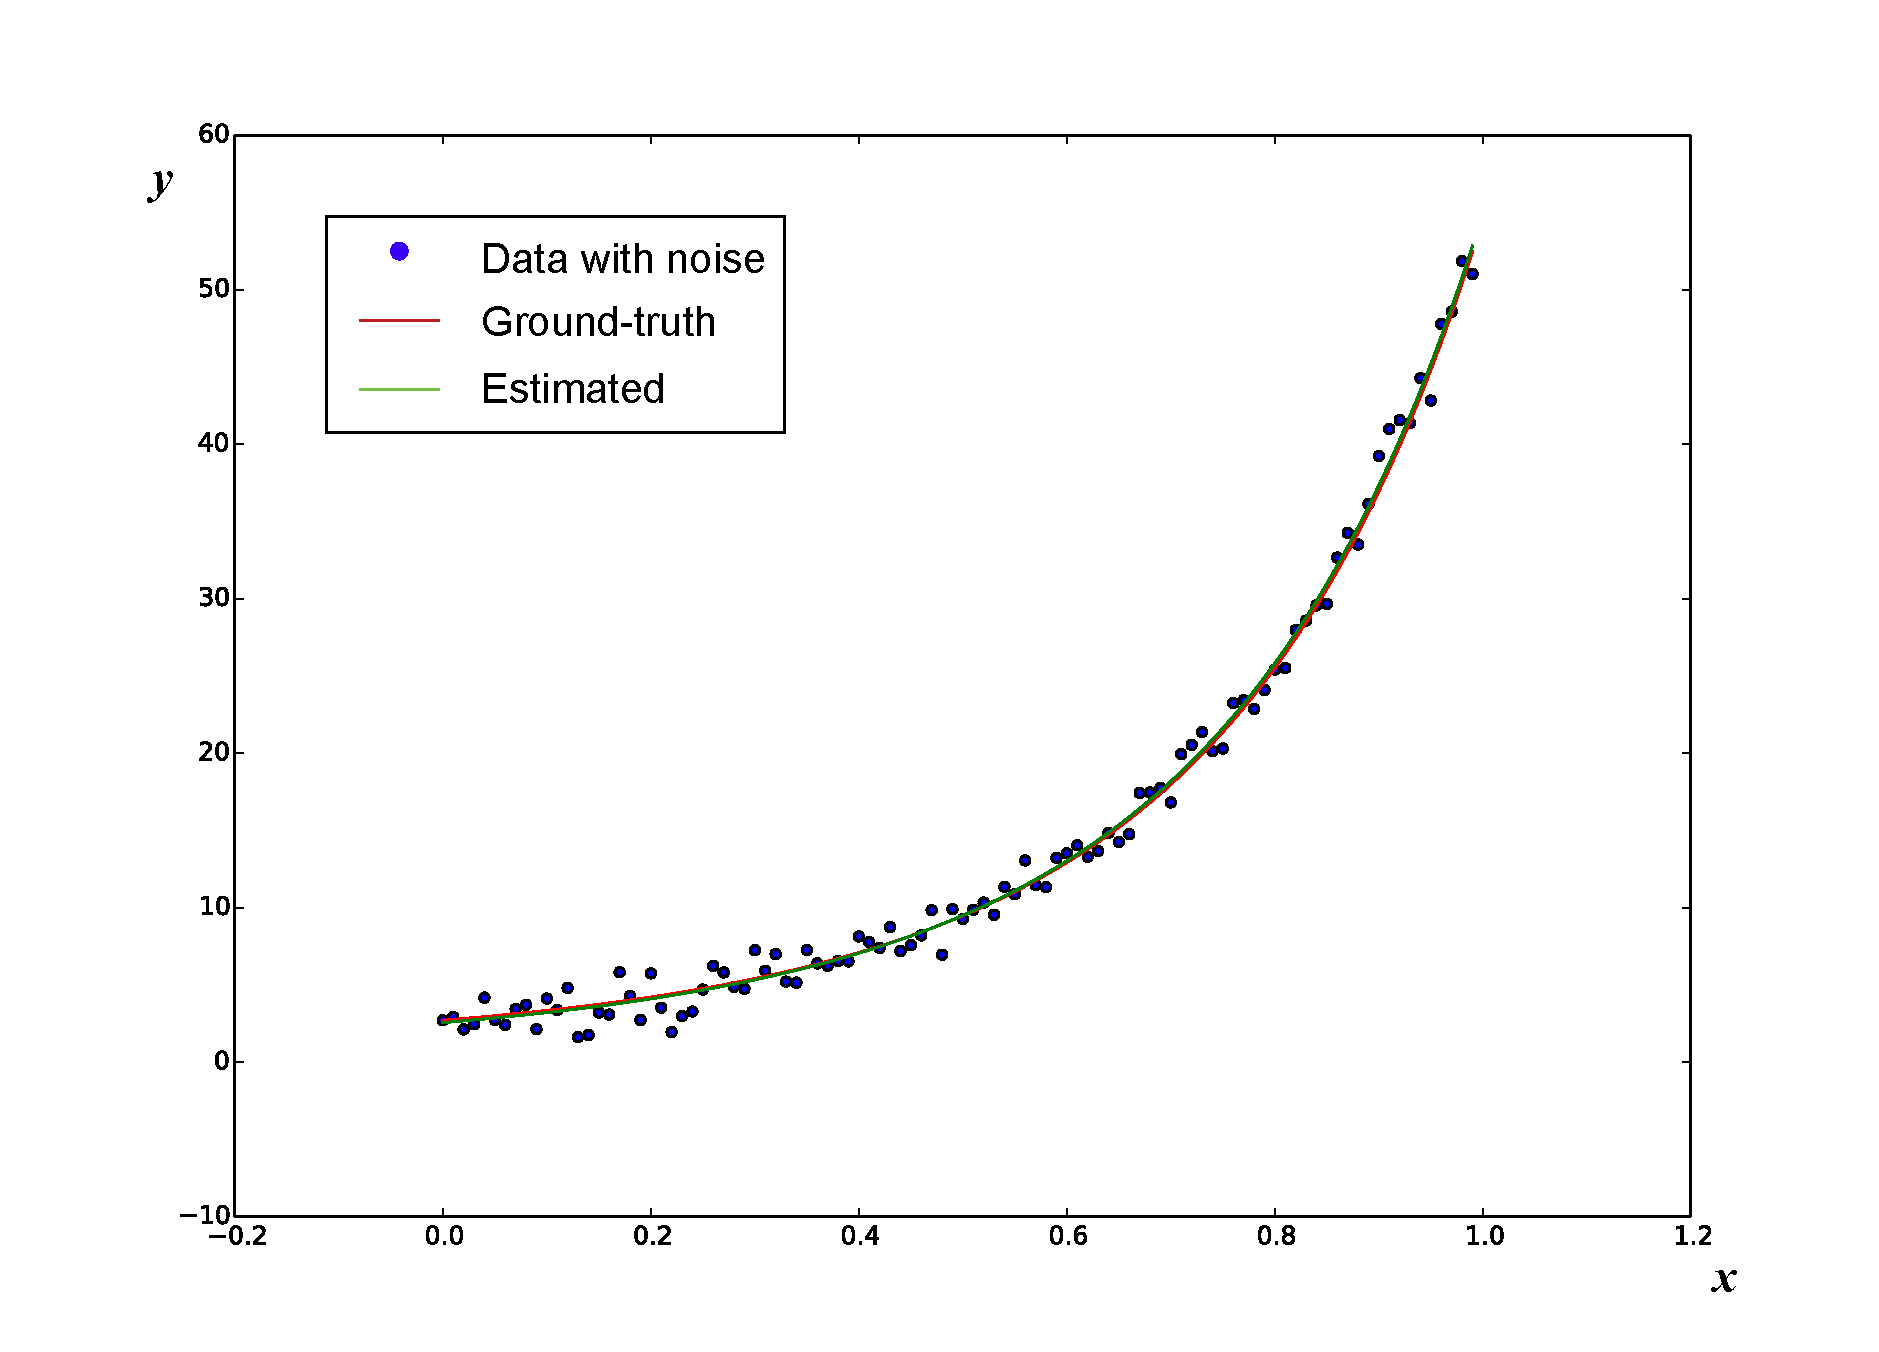
\includegraphics[width=0.8\textwidth]{optimization/ceresFitting.pdf}
    \caption{Estimated curve when the noise $\sigma=1$. }
    \label{fig:ceres-fitting}
\end{figure}

\subsection{Curve Fitting with Google Ceres}
In the next two sections we introduce two C++ optimization libraries: the Ceres library \cite{Ceres} from Google and the g2o library \cite{Kummerle2011} based on graph optimization. Since in g2o, we still need some knowledge about graph optimizations, we first go through the Ceres here, then introduce some graph optimization theories, and finally talk about g2o. Since the optimization algorithms will still appear in the later chapters, please make sure you understand the meaning of the optimization algorithm and the content of the program.

\subsubsection{Introduction to Ceres}
Google Ceres is a widely used optimization library for least-square problems. In Ceres, as users, we only need to define the optimization problem to be solved according to specific steps and then hand it over to the solver for calculation. The most general form of the least-square problem solved by Ceres is as follows (kernel function least-squares with boundary):
\begin{equation}
    \begin{array}{ll}
        \min \limits_x \quad & \frac{1}{2}\sum\limits_i {{\rho _i}\left( {{{\left\| {{f_i}\left( {{x_{{i_1}}}, \cdots {x_{{i_n}}}} \right)} \right\|}^2}} \right)} \\
        \mathrm{s.t.} \quad & {l_j} \leqslant {x_j} \leqslant {u_j}.
    \end{array}
\end{equation}

In this question, $x_1, \cdots, x_n$ are optimized variables, also called parameter blocks, $f_i$ is called cost function, or residual blocks. $l_j$ and $u_j$ are the upper and lower limits of the $j$-th optimization variable. In the simplest case, we can set $l_j = -\infty, u_j=\infty$ (do not limit the boundary of the optimization variable). At this time, the objective function is composed of many square terms after the kernel function $\rho(\cdot)$ and then the sum \footnote{Kernel function is discussed in chapter \ref{cpt:backend1}. }. Similarly, you can take $\rho$ as the identity function. The objective function is the sum of the squares of many terms.

In order to tell Ceres the definition of the problem, we need to do the following things:
\begin{enumerate}
    \item Defines each parameter block. The parameter block is usually a trivial vector, but it can also be defined as a particular structure such as quaternion and Lie algebra in SLAM. If it is a vector, we need to allocate a double array for each parameter block to store the variable's value.
    \item Then, define the calculation method of the residual block. The residual block is usually associated with several parameter blocks, performs some custom calculations on them, and then returns the residual value. After that, Ceres will sum the squares residuals, which is used as the overall objective function.
    \item In the residual blocks, we also need to define the Jacobian calculation method. In Ceres, we can use the ``automatic derivative'' function or manually specify the Jacobian calculation process. If you want to use automatic derivation, then the residual block must be written in a specific way: the residual calculation should be implemented as a bracketed operator with a template. We will illustrate this point through an example.
    \item Finally, add all the parameter blocks and residual blocks to Ceres's Problem object and call the Solve function to solve it. Before solving, we can pass some configuration information, such as the number of iterations, termination conditions, etc., or use the default configuration.
\end{enumerate}
Next, let's actually operate Ceres to solve the curve-fitting problem and understand the optimization process.

\subsubsection{Install Ceres}
In order to use Ceres, we first need to compile and install it. Ceres' GitHub address is \url{https://github.com/ceres-solver/ceres-solver}, and you can also directly use Ceres in our 3rdparty directory of the code repository so that you will use the same version as mine.

Like the libraries encountered before, Ceres is also a CMake project. Before compiling it, we need to install the dependencies first. You can install them with apt-get in Ubuntu, mainly some logging and testing tools used by Google:
\begin{lstlisting}[language=sh,caption=Terminal input: ]
sudo apt-get install liblapack-dev libsuitesparse-dev libcxsparse3 libgflags-dev libgoogle-glog-dev libgtest-dev 
\end{lstlisting}

Then, enter the Ceres library directory, use cmake to compile and install it. We have done this process many times, so I won't repeat it here. After the installation is complete, we can find the Ceres header file under /usr/local/include/ceres, and find the library file named libceres.a under /usr/local/lib/. With these files, we are able to include the Ceres headers and do the optimization calculations.

\subsubsection{Use Ceres for Curve Fitting}
The following code demonstrates how to use Ceres to solve the same problem.
\begin{lstlisting}[language=c++,caption=slambook/ch6/ceresCurveFitting.cpp]
#include <iostream>
#include <opencv2/core/core.hpp>
#include <ceres/ceres.h>
#include <chrono>

using namespace std;

// residual
struct CURVE_FITTING_COST {
    CURVE_FITTING_COST(double x, double y) : _x(x), _y(y) {}
    
    // implement operator () to compute the error
    template<typename T>
    bool operator()(
        const T *const abc, // the estimated variables, 3D vector
        T *residual) const {
        // y-exp(ax^2+bx+c)
        residual[0] = T(_y) - ceres::exp(abc[0] * T(_x) * T(_x) + abc[1] * T(_x) + abc[2]);
        return true;
    }
    
    const double _x, _y;    // x,y data 
};

int main(int argc, char **argv) {
    // same as before
    double ar = 1.0, br = 2.0, cr = 1.0;         // ground-truth values
    double ae = 2.0, be = -1.0, ce = 5.0;        // initial estimation
    int N = 100;                                 // num of data points
    double w_sigma = 1.0;                        // sigma of the noise
    double inv_sigma = 1.0 / w_sigma;
    cv::RNG rng;                                 // Random number generator 
    
    vector<double> x_data, y_data;      // the data
    for (int i = 0; i < N; i++) {
        double x = i / 100.0;
        x_data.push_back(x);
        y_data.push_back(exp(ar * x * x + br * x + cr) + rng.gaussian(w_sigma * w_sigma));
    }
    
    double abc[3] = {ae, be, ce};
    
    // construct the problem in ceres
    ceres::Problem problem;
    for (int i = 0; i < N; i++) {
        problem.AddResidualBlock(     // add i-th residual into the problem
            // use auto-diff, template params: redisual type, output dimension, input dimension
            // shoule be same as the struct written before
            new ceres::AutoDiffCostFunction<CURVE_FITTING_COST, 1, 3>(
                new CURVE_FITTING_COST(x_data[i], y_data[i])
            ),
            nullptr,            // kernel function, don't use here
            abc                 // estimated variables
        );
    }
    
    // set the solver options
    ceres::Solver::Options options;     // actually there're lots of params can be adjusted
    options.linear_solver_type = ceres::DENSE_NORMAL_CHOLESKY;  // use cholesky to solve the normal equation
    options.minimizer_progress_to_stdout = true;   // print to cout
    
    ceres::Solver::Summary summary;                
    chrono::steady_clock::time_point t1 = chrono::steady_clock::now();
    ceres::Solve(options, &problem, &summary);  // do optimization!
    chrono::steady_clock::time_point t2 = chrono::steady_clock::now();
    chrono::duration<double> time_used = chrono::duration_cast<chrono::duration<double>>(t2 - t1);
    cout << "solve time cost = " << time_used.count() << " seconds. " << endl;
    
    // get the outpus
    cout << summary.BriefReport() << endl;
    cout << "estimated a,b,c = ";
    for (auto a:abc) cout << a << " ";
    cout << endl;
    
    return 0;
}
\end{lstlisting}

The code is quite self-explained because we write a lot of comments here. As you can see, we used OpenCV's noise generator to generate 100 data with Gaussian noise and then used Ceres for fitting. The Ceres usage demonstrated here has the following steps:

\begin{enumerate}
    \item Defines the class of the residual block. The method is to write a class (or structure) and define the () operator with template parameters in the class to become a functor. \footnote{The functor is a C++ term. Such a class can be called as if it were a function because the operator () is overloaded.}  This definition allows Ceres to call the <double>() method for an instance of this class like a function. In fact, Ceres will pass the Jacobian matrix as a type parameter to this function to realize automatic derivation (auto-diff, which is one of the best features of Ceres).
    
    \item The double array abc[3] in the program is the parameter block. We construct a CURVE\_FITTING\_COST object for each data for the residual block and then call AddResidualBlock to add the error term to the objective function. Since the optimization requires gradients, we have several options: (1) Use Ceres's auto diff feature. (2) Use numeric diff \footnote{Automatic derivation is also implemented with numerical derivatives, but since it is a template operation, it runs faster. }; (3) Derive the analytical derivative form by yourself and provide it to Ceres. Because automatic derivation is the most convenient in coding, we use automatic derivation here.
    
    \item Automatic derivation requires specifying the dimensions of the error term and optimization variable. The error here is a scalar with a dimension of 1; the optimized three quantities are $a, b, c$ with 3. Therefore, the variable dimensions are set to 1, 3 in the template parameter of the auto-derivation class AutoDiffCostFunction.
    
    \item After setting the problem, call the Solve function to solve it. You can configure (very detailed) optimization options in Ceres. For example, you can choose to use line search or trust region, the number of iterations, step size, and so on. Readers can check the Ceres options to see what optimization methods are available. Of course, the default configuration can be used for a wide range of problems.
\end{enumerate}

Finally, let's see the experimental results by calling build/ceresCurveFitting: 
\begin{lstlisting}[caption=erminal output: ]
    iter      cost      cost_change  |gradient|   |step|    tr_ratio  tr_radius  ls_iter  iter_time  total_time
    0  1.597873e+06    0.00e+00    3.52e+06   0.00e+00   0.00e+00  1.00e+04        0    2.10e-05    7.92e-05
    1  1.884440e+05    1.41e+06    4.86e+05   9.88e-01   8.82e-01  1.81e+04        1    5.60e-05    1.05e-03
    2  1.784821e+04    1.71e+05    6.78e+04   9.89e-01   9.06e-01  3.87e+04        1    2.00e-05    1.09e-03
    3  1.099631e+03    1.67e+04    8.58e+03   1.10e+00   9.41e-01  1.16e+05        1    6.70e-05    1.16e-03
    4  8.784938e+01    1.01e+03    6.53e+02   1.51e+00   9.67e-01  3.48e+05        1    1.88e-05    1.19e-03
    5  5.141230e+01    3.64e+01    2.72e+01   1.13e+00   9.90e-01  1.05e+06        1    1.81e-05    1.22e-03
    6  5.096862e+01    4.44e-01    4.27e-01   1.89e-01   9.98e-01  3.14e+06        1    1.79e-05    1.25e-03
    7  5.096851e+01    1.10e-04    9.53e-04   2.84e-03   9.99e-01  9.41e+06        1    1.81e-05    1.28e-03
    solve time cost = 0.00130755 seconds. 
    Ceres Solver Report: Iterations: 8, Initial cost: 1.597873e+06, Final cost: 5.096851e+01, Termination: CONVERGENCE
    estimated a,b,c = 0.890908 2.1719 0.943628 
\end{lstlisting}

The final optimized value is basically the same as our experimental result in the previous section, but Ceres is relatively slow in running speed. Ceres used about 1.3 milliseconds on my machine, which is about six times slower than the handwritten Gauss-Newton method.

I hope readers have a general understanding of how to use Ceres through this simple example. Its advantage is that it provides an automatic derivation tool, making it unnecessary to calculate the troublesome Jacobian matrix. Ceres's automatic derivation is realized through template elements, and the automatic derivation can be completed at compile-time, but it is still a numerical derivative. Most of the time in this book, I will still introduce the Jacobian matrix calculation because it helps understand the problem. Besides, Ceres' optimization process configuration is also very rich, making it suitable for a wide range of least-squares optimization problems, including various problems other than SLAM.

\subsection{Curve Fitting with G2o}
The second practice part of this lecture is about another optimization library (widely used mainly in the SLAM field): g2o (general graphic optimization, g$^2$o). It is a library based on \textit{graphic optimization}. Graph optimization is a theory that combines nonlinear optimization with graph theory, so before using it, let's spend a little space to introduce graph optimization theory.

\subsubsection{Introduction to Graph Optimization Theory}
We have introduced the solution of nonlinear least-squares. The least-square problem in SLAM is normally composed of the sum of many small error terms. However, if we only treat them as variables and residuals, it would be hard to tell the \textit{relationship} between them. For example, how many error terms are related to a certain optimization variable $x_j$? If we adjust some variables, does the overall cost function change or keep the same? Furthermore, we hope to visually see what optimization problem \textit{looks like}. Therefore, graph optimization is involved.

Graph optimization is a way to express the optimization problem as a graph.  A graph consists of a number of vertices and edges connecting these vertices. A  vertex is used to represent an optimization variable, and an edge is used to represent an error term. Therefore, for any of the above-mentioned nonlinear least-squares problems, we can construct a corresponding graph. We can simply call it a graph or use the probability graph definition, call it a Bayesian graph or a factor graph. Sometimes it is also called a hypergraph because an edge can be connected to more than two variables, e.g., where an error term is related to more than two variables. 

\autoref{fig:graph-optimization}~ is a simple graph optimization example. We use triangles to represent the camera poses and circles to represent landmark points, which constitute the vertices. At the same time, the solid line represents the camera's motion model, and the dashed line represents the observation model, which forms the edges of the graph optimization. At this point, although the mathematical form of the entire problem is still like \eqref{eq:least-square}, now we can intuitively see the structure of the problem. If you want, you can also make improvements like removing isolated vertices or preferentially optimizing vertices with more edges (or, in graph theory terms, greater degrees). But the most basic idea is just to use a graph model to express a nonlinear least-squares optimization problem. And we can use some properties of the graph model to do better optimization.

\begin{figure}[!ht]
    \centering
    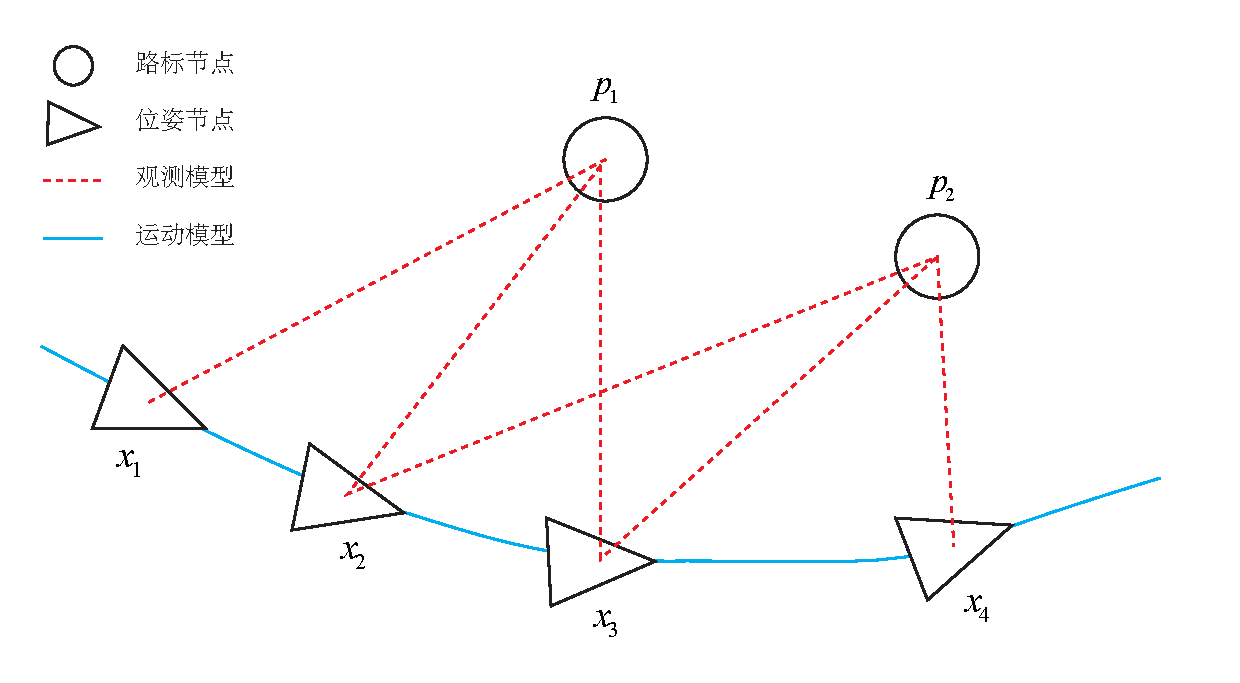
\includegraphics[width=1.0\textwidth]{optimization/graphOptimization.pdf}
    \caption{An example of the graph optimization.}
    \label{fig:graph-optimization}
\end{figure}

The g2o is a \textit{general} graph optimization library. ``General'' means that you can solve any least-squares problem that can be expressed as graph optimization, obviously including the curve-fitting problem discussed above. Let us demonstrate how to do that.

\subsubsection{Compilation and Installation of G2o}
Just like the Ceres section, we should first compile and install the g2o library. Readers should have experienced this process many times, and they are basically the same. Regarding g2o, readers can download it from GitHub: \url{https://github.com/RainerKuemmerle/g2o}, or obtain it from the third-party code library provided in this book. Since g2o is still being updated, I suggest using g2o under 3rdparty to ensure that the version is the same as mine.

G2o is also a cmake project. Let's install its dependencies first (some dependencies overlap with Ceres):
\begin{lstlisting}[language=sh,caption=Terminal input:]
    sudo apt-get install qt5-qmake qt5-default libqglviewer-dev-qt5 libsuitesparse-dev libcxsparse3 libcholmod3
\end{lstlisting}

Then, compile and install g2o according to the cmake method. The description of the process is omitted here. After the installation is complete, the header files of g2o will be located under /usr/local/g2o, and the library files will be located under /usr/local/lib/. We reconsider the curve fitting experiment in the Ceres routine and do that experiment again in g2o.

\subsubsection{Curve Fitting with G2o}
In order to use g2o, the curve fitting problem must first be constructed into graph optimization. In this process, just remember that nodes are the optimization variables, and edges are the error terms. The graph optimization problem of curve fitting can be drawn in the form of \autoref{fig:graph-fitting}~.

\begin{figure}[!ht]
    \centering
    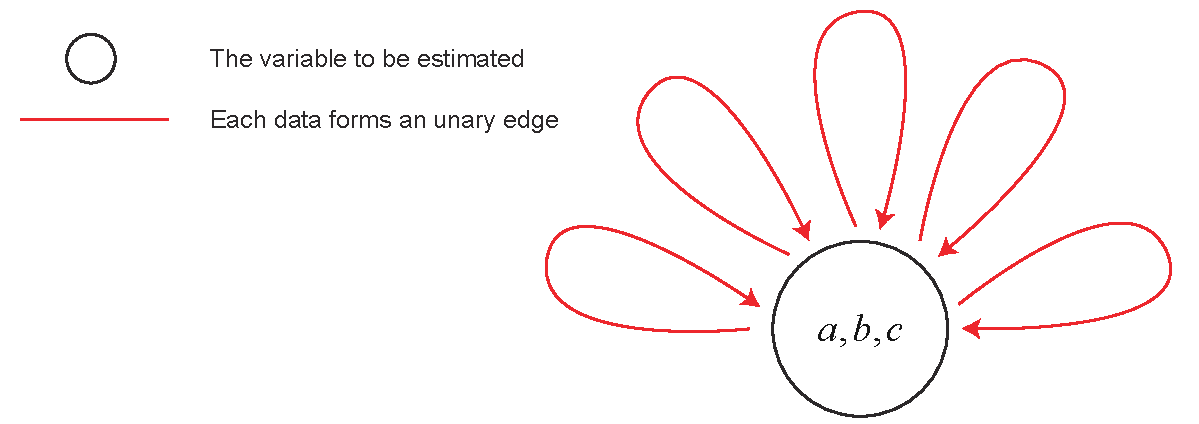
\includegraphics[width=.9\textwidth]{optimization/graphFitting.pdf}
    \caption{Graph model of the curve fitting problem. }
    \label{fig:graph-fitting}
\end{figure}

The entire problem has only one vertex: the parameters $a, b, c$ of the curve model. Each noisy data point constitutes an error term, which is the edge of the graph optimization. But the edges here are not the same as we usually think. They are unary edges, which means that the edges connect only one vertex. Because the entire graph has only one vertex. So in \autoref{fig:graph-fitting}~, we can only draw it as if it is connected to itself. An edge in graph optimization can connect one, two, or more vertices, reflecting how many optimization variables each error is related to. In a slightly mysterious way, we call it a hyperedge. The whole graph is called hypergraph \footnote{I personally would better call it just as a graph to avoid being mysterious. }.

After clarifying the graph model, the next step is to build the model in g2o for optimization. As a user of g2o, what we need to do mainly includes the following steps:
\begin{enumerate}
    \item Define the type of vertices and edges.
    \item Build the graph.
    \item Select the optimization algorithm.
    \item Call g2o to optimize and get the result.
\end{enumerate}

This part is very similar to Ceres. Of course there will be some differences in coding. Let's demonstrate the program.
\begin{lstlisting}[language=c++,caption=slambook/ch6/g2oCurveFitting.cpp]
#include <iostream>
#include <g2o/core/g2o_core_api.h>
#include <g2o/core/base_vertex.h>
#include <g2o/core/base_unary_edge.h>
#include <g2o/core/block_solver.h>
#include <g2o/core/optimization_algorithm_levenberg.h>
#include <g2o/core/optimization_algorithm_gauss_newton.h>
#include <g2o/core/optimization_algorithm_dogleg.h>
#include <g2o/solvers/dense/linear_solver_dense.h>
#include <Eigen/Core>
#include <opencv2/core/core.hpp>
#include <cmath>
#include <chrono>

using namespace std;

// vertex: 3d vector 
class CurveFittingVertex : public g2o::BaseVertex<3, Eigen::Vector3d> {
public:
    EIGEN_MAKE_ALIGNED_OPERATOR_NEW
    
    // override the reset function
    virtual void setToOriginImpl() override {
        _estimate << 0, 0, 0;
    }
    
    // override the plus operator, just plain vector addition
    virtual void oplusImpl(const double *update) override {
        _estimate += Eigen::Vector3d(update);
    }
    
    // the dummy read/write function
    virtual bool read(istream &in) {}
    virtual bool write(ostream &out) const {}
};

// edge: 1D error term, connected to exactly one vertex
class CurveFittingEdge : public g2o::BaseUnaryEdge<1, double, CurveFittingVertex> {
public:
    EIGEN_MAKE_ALIGNED_OPERATOR_NEW
    
    CurveFittingEdge(double x) : BaseUnaryEdge(), _x(x) {}
    
    // define the error term computation
    virtual void computeError() override {
        const CurveFittingVertex *v = static_cast<const CurveFittingVertex *> (_vertices[0]);
        const Eigen::Vector3d abc = v->estimate();
        _error(0, 0) = _measurement - std::exp(abc(0, 0) * _x * _x + abc(1, 0) * _x + abc(2, 0));
    }
    
    // the jacobian
    virtual void linearizeOplus() override {
        const CurveFittingVertex *v = static_cast<const CurveFittingVertex *> (_vertices[0]);
        const Eigen::Vector3d abc = v->estimate();
        double y = exp(abc[0] * _x * _x + abc[1] * _x + abc[2]);
        _jacobianOplusXi[0] = -_x * _x * y;
        _jacobianOplusXi[1] = -_x * y;
        _jacobianOplusXi[2] = -y;
    }
    
    virtual bool read(istream &in) {}
    virtual bool write(ostream &out) const {}
public:
    double _x;  // x data, note y is given in _measurement
};

int main(int argc, char **argv) {
    // ... we omit the data sampling code, same as before
    typedef g2o::BlockSolver<g2o::BlockSolverTraits<3, 1>> BlockSolverType;  // bolck solver 
    typedef g2o::LinearSolverDense<BlockSolverType::PoseMatrixType> LinearSolverType; // linear solver
    
    // choose the optimizatoin method from GN, LM, DogLeg 
    auto solver = new g2o::OptimizationAlgorithmGaussNewton(
        g2o::make_unique<BlockSolverType>(g2o::make_unique<LinearSolverType>()));
    g2o::SparseOptimizer optimizer;    // graph optimizer
    optimizer.setAlgorithm(solver);    // set the algorithm
    optimizer.setVerbose(true);        // print the results
    
    // add vertex
    CurveFittingVertex *v = new CurveFittingVertex();
    v->setEstimate(Eigen::Vector3d(ae, be, ce));
    v->setId(0);
    optimizer.addVertex(v);
    
    // add edges
    for (int i = 0; i < N; i++) {
        CurveFittingEdge *edge = new CurveFittingEdge(x_data[i]);
        edge->setId(i);
        edge->setVertex(0, v);                // connect to the vertex
        edge->setMeasurement(y_data[i]);      // measurement
        edge->setInformation(Eigen::Matrix<double, 1, 1>::Identity() * 1 / (w_sigma * w_sigma)); // set the information matrix
        optimizer.addEdge(edge);
    }
    
    // carry out the optimization
    cout << "start optimization" << endl;
    chrono::steady_clock::time_point t1 = chrono::steady_clock::now();
    optimizer.initializeOptimization();
    optimizer.optimize(10);
    chrono::steady_clock::time_point t2 = chrono::steady_clock::now();
    chrono::duration<double> time_used = chrono::duration_cast<chrono::duration<double>>(t2 - t1);
    cout << "solve time cost = " << time_used.count() << " seconds. " << endl;
    
    // print the results
    Eigen::Vector3d abc_estimate = v->estimate();
    cout << "estimated model: " << abc_estimate.transpose() << endl;
    
    return 0;
}
\end{lstlisting}

In this program, we derive graph optimization vertices and edges for curve fitting from g2o built-in classes: CurveFittingVertex and CurveFittingEdge, which essentially expands the use of g2o. These two classes are derived from BaseVertex and BaseUnaryEdge, respectively. In the derived classes, we have rewritten some important virtual functions:
\begin{enumerate}
    \item Vertex update function: \textit{oplusImpl}. We know that the most important thing in the optimization process is the calculation of incremental $\Delta \mathbf{x}$, and this function deals with $\mathbf{x}_{k+1} = \mathbf{x}_k + \Delta \mathbf{x}$ process.

    Readers may think this is not something worth mentioning because it is just simple addition. Why doesn't g2o help us complete it? In the curve fitting process, since the optimization variables (curve parameters) are located in the plain vector space, this update calculation is indeed nothing but just simple addition. However, when the optimization variable is not in the vector space, for example, for $\mathbf{x}$ is the camera pose, it does not necessarily have an addition operation. At this time, it is necessary to redefine the behavior of how the increment is added to the existing estimate. According to the explanation in lecture \ref{cpt:4}, we may use the left-multiplication update or the right-multiplication update instead of direct addition.

    \item Vertex reset function: \textit{setToOriginImpl}. This is trivial, and we just set the estimate to zero.

    \item The error calculation function: computeError. According to the curve model, this function needs to take out the current estimated value of the vertex connected by the edge and compare it with its observed value. This is consistent with the error model in the least-squares problem.
    
    \item The Jacobian calculation function: \textit{linearizeOplus}. In this function, we calculate the Jacobian of each edge relative to the vertex.

    \item Save and read functions: read, write. Since we do not want to perform read/write operations, leave it blank.
\end{enumerate}

After defining the vertices and edges, we declare a graph model in the main function, then add vertices and edges to the graph model according to the generated noise data, and finally call the optimization function for optimization. g2o will give the optimized result:
\begin{lstlisting}[language=sh,caption=Terminal output:]
start optimization
iteration= 0	 chi2= 376785.128234	 time= 3.3299e-05	 cumTime= 3.3299e-05	 edges= 100	 schur= 0
iteration= 1	 chi2= 35673.566018	 time= 1.3789e-05	 cumTime= 4.7088e-05	 edges= 100	 schur= 0
iteration= 2	 chi2= 2195.012304	 time= 1.2323e-05	 cumTime= 5.9411e-05	 edges= 100	 schur= 0
iteration= 3	 chi2= 174.853126	 time= 1.3302e-05	 cumTime= 7.2713e-05	 edges= 100	 schur= 0
iteration= 4	 chi2= 102.779695	 time= 1.2424e-05	 cumTime= 8.5137e-05	 edges= 100	 schur= 0
iteration= 5	 chi2= 101.937194	 time= 1.2523e-05	 cumTime= 9.766e-05	 edges= 100	 schur= 0
iteration= 6	 chi2= 101.937020	 time= 1.2268e-05	 cumTime= 0.000109928	 edges= 100	 schur= 0
iteration= 7	 chi2= 101.937020	 time= 1.2612e-05	 cumTime= 0.00012254	 edges= 100	 schur= 0
iteration= 8	 chi2= 101.937020	 time= 1.2159e-05	 cumTime= 0.000134699	 edges= 100	 schur= 0
iteration= 9	 chi2= 101.937020	 time= 1.2688e-05	 cumTime= 0.000147387	 edges= 100	 schur= 0
solve time cost = 0.000919301 seconds. 
estimated model: 0.890912   2.1719 0.943629
\end{lstlisting}

We use the Gauss-Newton method for gradient descent, and after 9 iterations, the optimization result is obtained, which is almost the same as the Ceres and handwritten Gauss-Newton method. From the running speed perspective, our experimental conclusion is that handwriting is faster than g2o, and g2o is faster than Ceres. This is a generally intuitive experience that versatility and efficiency are often contradictory. However, in this experiment, Ceres uses automatic derivation, and the solver configuration is not completely consistent with Gauss-Newton, so it seems slower.

\section{Summary}
This section introduces a nonlinear optimization problem often encountered in SLAM: the least-squares problem consisting of the sum of squares of many error terms. We introduced its definition and solution and discussed two main gradient descent methods: the Gauss-Newton method and the Levenberg-Marquardt method. In the practice part, two optimization libraries of the handwritten Gauss-Newton method, Ceres and g2o, were used to solve the same curve-fitting problem and found that they gave similar results.

Since the bundle adjustment has not been discussed in detail, we have chosen a simple but representative example of curve fitting in the practice part to demonstrate the general nonlinear least-squares solution method. In particular, if you use g2o to fit a curve, you must first convert the problem to graph optimization and define new vertices and edges. This approach is somewhat roundabout—the main purpose of g2o is not here. In contrast, Ceres' usage is much more natural because it is designed to be a general optimization library. However, the SLAM problem is about solving an optimization problem with many camera poses and many spatial points. In particular, when the camera pose is represented by Lie algebra, calculating the derivative of the camera pose in the error term will be worthy of detailed discussion. We will find in the follow-up content that g2o provides a large number of ready-to-use vertices and edges, which is very convenient for the camera pose estimation problem. In Ceres, we have to implement each cost function by ourselves, which has some inconveniences.

In the two programs of the practical part, we did not calculate the derivative of the curve model with respect to the three parameters but used the numerical derivative of the optimization library, which made the theory and code simpler. The Ceres library provides automatic derivation based on template elements and numerical derivation at runtime, while g2o only provides a numerical derivation method. However, for most problems, if you can derive the analytical form of the Jacobian matrix and tell the optimization library, you can avoid many problems in numerical derivation.

Finally, I hope readers can adapt to Ceres and g2o's extensive use of template programming. It may seem scary at first (especially the parenthesis operator for Ceres to set the residual block and the code for the g2o initialization part). But once you are familiar with it, you will feel that this method is natural and easy to extend. We will continue to discuss issues such as sparsity, kernel functions, and pose graphs in the SLAM backend lecture.

\section*{Exercises}
\begin{enumerate}
    \item Prove that in the linear equation $\mathbf{A} \mathbf{x} = \mathbf{b}$, when the coefficient matrix $\mathbf{A}$ is over-determined, the least-square solution is $\mathbf{x} = (\mathbf{A}^T\mathbf{A})^{-1}\mathbf{A}^T \mathbf{b}$.
    \item Investigate the advantages and disadvantages of the steepest descent method, Newton method, Gauss-Newton method, and Levenberg-Marquardt method. In addition to the Ceres library and g2o library we cited, are there any commonly used optimization libraries? (You may find some libraries on MATLAB.)
    \item Why does the coefficient matrix of the Gauss-Newton method's incremental equation may not be positive definite? What is the geometric meaning of indefinite? Why is the solution unstable in this case?
    \item What is DogLeg? What are the similarities and differences between it and the Gauss-Newton method and the Levenberg-Marquardt method? Please search for relevant materials \footnote{\url{http://www.numerical.rl.ac.uk/people/nimg/course/lectures/raphael/lectures/lec7slides.pdf}. }.
    \item Read Ceres' tutorials (\url{http://ceres-solver.org/tutorial.html}) to better understand its usage.
    \item Read the documentation that comes with g2o, can you understand it? If you still can't fully understand it, please come back after lectures \ref{cpt:backend1} and \ref{cpt:backend2}.
    \item[\optional] Please change the curve model in the curve fitting experiment, and use Ceres and g2o to optimize it. For example, write an example with more parameters and more complex models.
\end{enumerate}